\documentclass{standalone}
\usepackage{tikz}
\begin{document}
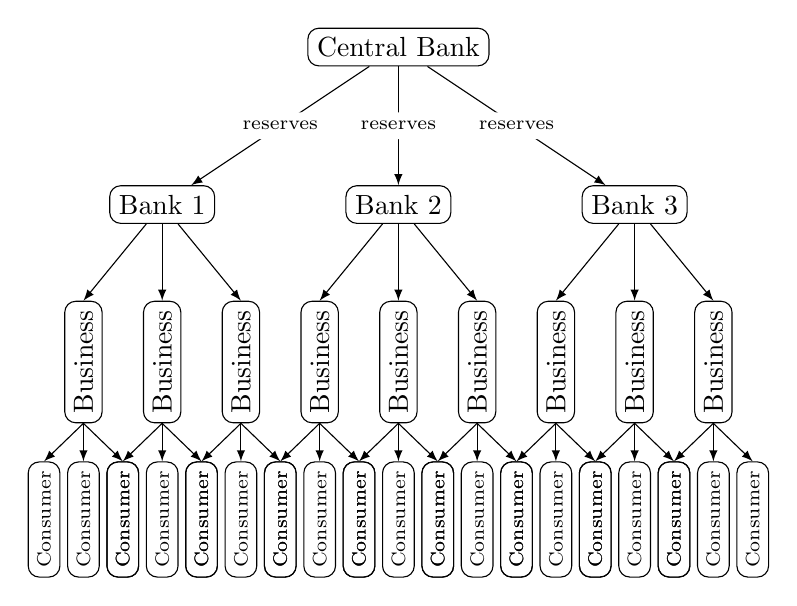
\begin{tikzpicture}
    \tikzset{
      pics/carc/.style args={#1:#2:#3}{
        code={
          \draw[pic actions] (#1:#3) arc(#1:#2:#3);
        }
      }
    }
    \tikzset{
        every node/.style={
            draw, rounded corners
        }
    }
    \node (cb) at (0,1) {Central Bank};
    \foreach [count=\i] \mybank in {-3,0,3}
    {
        \node (mybank\i) at (\mybank,-1) {Bank \i};
        \draw[->,>=latex] (cb) -- node[fill=white,draw=none] {\scriptsize reserves} (mybank\i) ;
        \foreach[count=\ii] \myclient in {-1,0,1}
        {
            \node[rotate=90] (myclient\ii) at (\mybank+\myclient,-3) {Business};
            \draw[<-,>=latex] (myclient\ii.east) -- (mybank\i);
            \foreach[count=\iii] \mycustomer in {-0.5,0,0.5}
            {
                \node[rotate=90] (mycustomer\iii) at (\mybank+\myclient+\mycustomer,-5) {\scriptsize Consumer};
                \draw[<-,>=latex] (mycustomer\iii.east) -- (myclient\ii.west);
            }
        }
    }   

\end{tikzpicture}
\end{document}